% !TeX spellcheck = en_US
\newpage
\section{Instruction set architecture}
The ISA level is the classical boundary between SW and HW and defines what is visible or not to the user. High level languages are translated into instructions from the ISA.

\subsection{CISC}
Complex Instruction Set Computer exist for chips, high programming languages and special purpose applications that favor complex instructions.\\
The \textbf{positive sides} are:
\begin{itemize}
	\item Execution of a single complex instruction is \textbf{faster} than the execution of a microprogram that does the same thing
	\item Shorter programs, thus \textbf{faster loading times}
	\item Direct \textbf{support of programming constructs} from higher programming languages
	\item Support of specialized \textbf{powerful compilers}
	\item \textbf{Compatibility}
	\item Support of \textbf{special purpose applications} (e.g. matrix operations)
\end{itemize}
The \textbf{negative sides}:
\begin{itemize}
	\item Needs faster main memories and the use of cache memory speed-up program execution
	\item Complex instructions can sometimes be \textbf{replaced with} several \textbf{simpler} and faster ones
	\item \textbf{Long development} cycle of CPUs
	\item \textbf{Complex control units}
	\item Large microprograms with potentially \textbf{more errors}
	\item Real programs often use only a small portion of the instructions
\end{itemize}

While there are many powerful instructions, usually just $20\%$ of them are used, still maintaining the complex format. Furthermore, many classical CISC architectures have a $\text{CPI}>2$.\\
That being said, optimized code for Pentium, Itanium and others usually have a $\text{CPI} \approx1$.

\subsection{RISC}
Reduced Instruction Set Computer consists of:
\begin{itemize}
	\item Few \textbf{instructions} ($\leq 128$)
	\item $\leq 4$ \textbf{instruction formats}
	\item Fixed \textbf{instruction length} of $32$ bit
	\item $\leq 4$ \textbf{addressing modes}
\end{itemize}
If possible all instructions should be implemented so that they can finish in a single cycle. As a consequence, there is no micro programming in RISC.

\begin{note}
	Early RISC processors had SW controlled pipeline (NOPs) instead of special hardware.
\end{note}
\subsubsection{Memory access}
This instruction set uses the \textbf{register/register} or \textbf{load/store} principle: \textbf{memory access} is possible only via \textit{load} and \textit{store} operations, while all other operations are done on registers.

\subsubsection{Pros and cons}
The \textbf{positive sides} are:
\begin{itemize}
	\item Single chip implementation, allowing the use of the saved \textbf{space} for something else
	\item Short development cycle
	\item \textbf{Higher clock rates}, \textbf{pipelines}
\end{itemize}
The main \textbf{downside} is the bottleneck in the memory interface, since main memory is much slower than internal registers and cache.

\subsection{Addressing modes}
There are different possibilities to calculate the address of an operand or the branch target address in the memory.
\subsubsection{Static}
The \textbf{classical} way is through an \textbf{absolute} address. This means that the location is determined at compilation and accessing dynamic structures requires a change in the address for each instruction.
\subsubsection{Dynamic}
In this case the calculation of the address is done at runtime: the instruction triggers the calculation of the \textbf{logical address} and then the memory management unit finds the physical one.
\begin{center}
	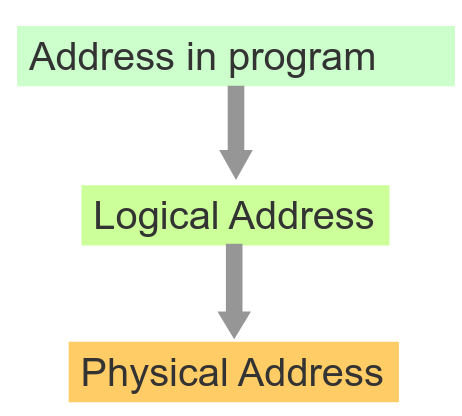
\includegraphics[scale=0.3]{dac}
\end{center}

\newpage
\subsection{Non linear execution}
Usually a program follows a non linear execution due to many reasons:
\begin{itemize}
	\item Jumps, branches
	\item Procedure calls, subroutines, method calls
	\item Multi-threading, parallel processing, co-routines
	\item Hardware interrupts
	\item Traps, software interrupts
\end{itemize}

\begin{figure}[!h]
	\centering
	\subfigure{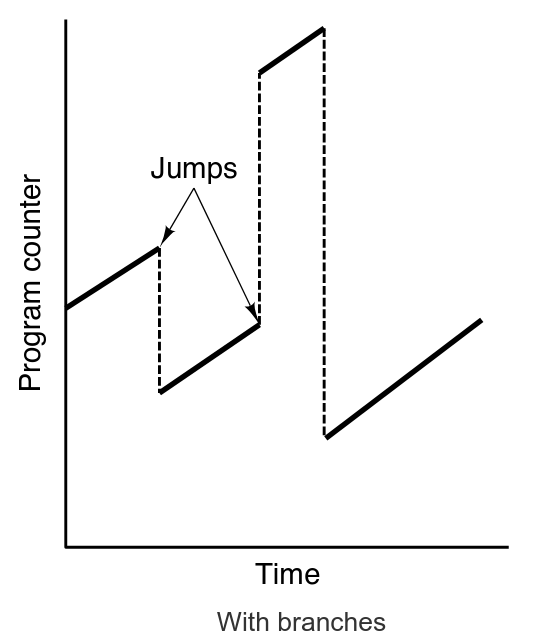
\includegraphics[scale=0.23]{branch}}
	\hfill
	\subfigure{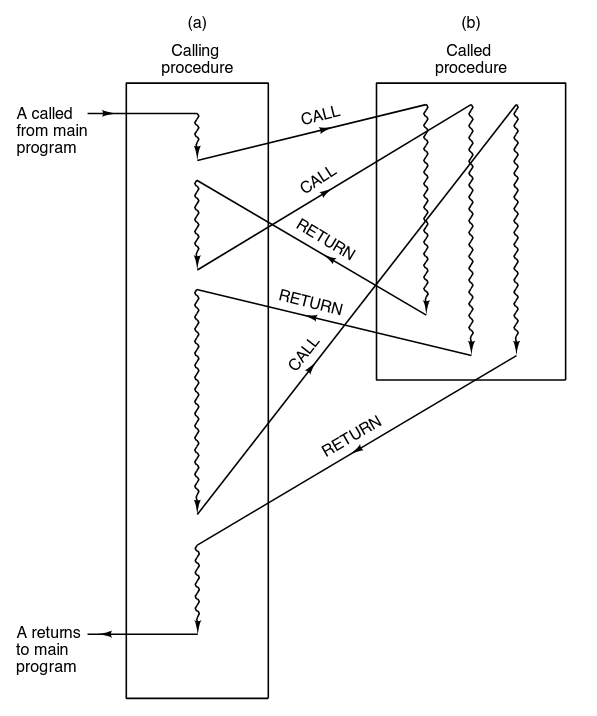
\includegraphics[scale=0.23]{procall}}
	\hfill
	\subfigure{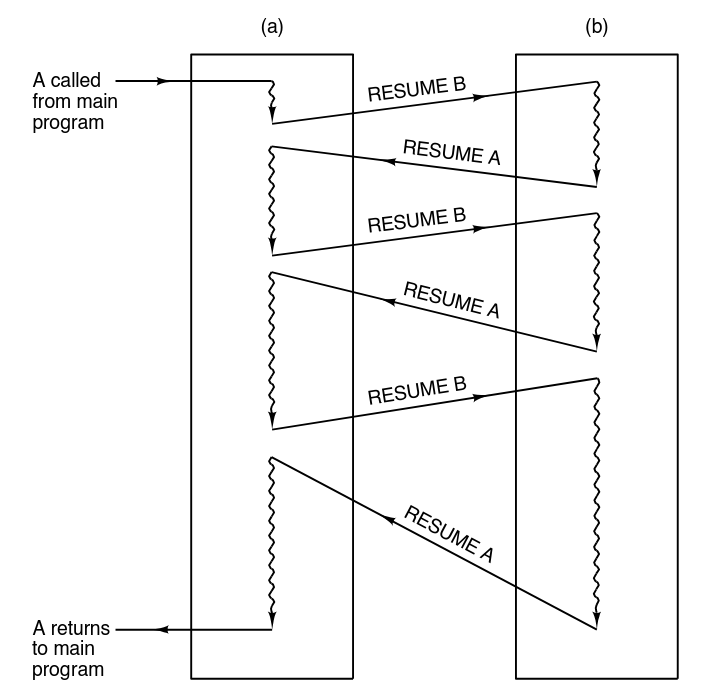
\includegraphics[scale=0.23]{corout}}
	\hfill
\end{figure}

\begin{definition}[Exception]
	Interruption of the programmed control flow of instructions during runtime.
\end{definition}
\subsubsection{Causes}
Exceptions may be caused by:
\begin{itemize}
	\item \textbf{External} reasons: asynchronous events such as
	\begin{itemize}
		\item \textit{RESET}: reset of the processor (e.g. power button)
		\item \textit{HALT}: stop the execution of the processor (e.g. to avoid conflict on memory access)
		\item \textit{ERROR}: call of an error routine (e.g. bus errors)
		\item \textbf{Interrupts}: request triggered by an external device (e.g. to announce incoming data). They can be \textit{maskable} or \textit{non maskable}
	\end{itemize}
	\item \textbf{Internal} reasons: synchronous events such as
	\begin{itemize}
		\item \textbf{Software interrupts}: \textit{INT} instructions in the program triggers an interrupt (e.g. system call)
		\item \textbf{Traps}: exception caused by internal events (e.g. overflow)
	\end{itemize}
\end{itemize}
\newpage
\subsubsection{Handling}
Handling of exceptions requires specialized routines called \textbf{Interrupt Service Routine} (ISR). They have the same structure as a subprogram but with some differences:
\begin{table}[!h]
	\centering
	\begin{tabular}{|p{2cm}|p{3cm}|p{3.5cm}|}
		\hline
		\textbf{Activity} & \textbf{Subprogram} & \textbf{ISR} \\
		\hline
		\textit{Activation} & \textit{call} subroutine & \textit{INT} instruction or hardware activation\\
		\hline
		\textit{Return after completion} & \textit{RET} instruction & \textit{RETI} instruction \\
		\hline
		\textit{Calculation of starting address} & Written in calling program & Determined via interrupt table \\
		\hline
		\textit{Saving status} & Typically saves PC on a stack & Saves PC and PSW on a stack\\
		\hline
	\end{tabular}
\end{table}

\noindent The \textbf{steps} of an ISR are:
\begin{enumerate}
	\item Interrupt activation
	\item Finalize the current instruction
	\item Check if SW or internal/external HW
	\item Check if \textit{Interrupt Enable} bit is set
	\item If HW, find the source and activate the acknowledge (INTA)
	\item Reset \textit{Interrupt Enable} to avoid additional interrupts
	\item Save PSW and PC on stack
	\item Calculate the start address and load it to PC. Usually done through the \textbf{Interrupt Vector Table}, which is at a specific location and contains the start addresses of the ISRs
	\begin{center}
		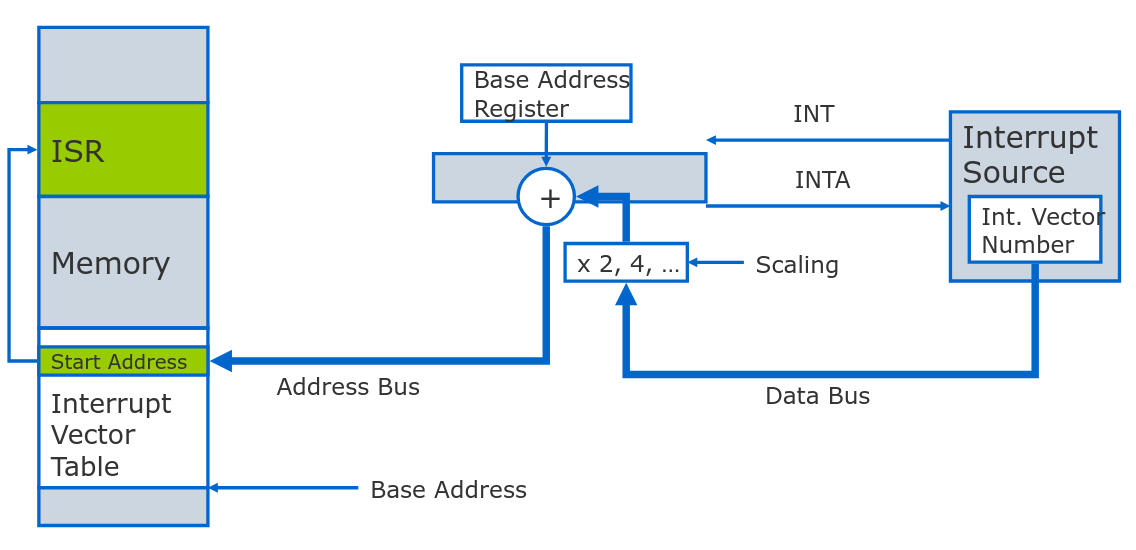
\includegraphics[scale=0.3]{isr}
	\end{center}
	\item Execute the ISR:
	\begin{itemize}
		\item Push the used register on stack
		\item Set the interrupt bit to allow more interrupts
		\item Execute ISR
		\item Pop the registers from stack
		\item Return using \textit{IRET}
	\end{itemize}
	\item Restore PSW and PC and continue the original program
\end{enumerate}

\subsubsection{Multiple interrupts}
During the handling of an interrupt, more may happen. There are two different approaches to handle them:
\begin{itemize}
	\item \textbf{Fair}: continue cyclic polling following the last served source, granting an equal chance of being served
	\begin{center}
		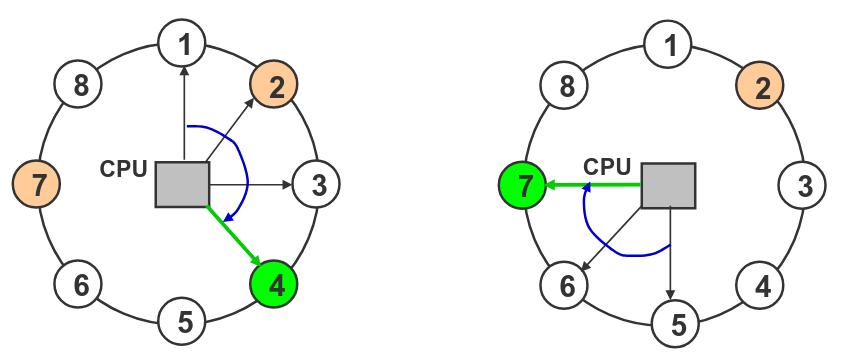
\includegraphics[scale=0.3]{fair}
	\end{center}
	\item \textbf{Priority}: cyclic polling always starts at a predetermined sourced. Every source gets a different priority and the higher one are served first.
	\begin{center}
		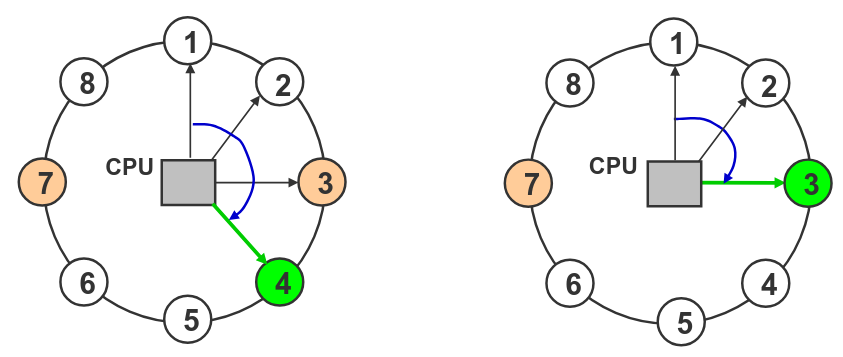
\includegraphics[scale=0.3]{priority}
	\end{center}
\end{itemize}
It's possible to use \textbf{hardware daisy chaining} to handle multiple interrupts, using specialized hardware for prioritization and identification of interrupts. Each source for an interrupt uses dedicated HW for connecting with a successor and a predecessor. The first one has the highest priority.
\begin{center}
	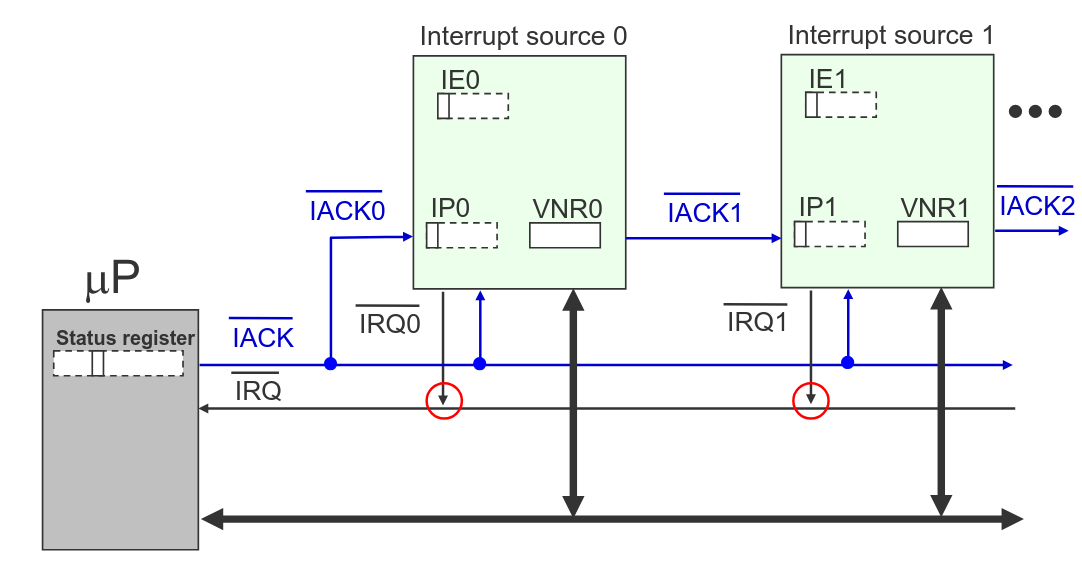
\includegraphics[scale=0.3]{daisychain}
\end{center}